\section{Stellar Nucleosynthesis in Massive Stars}

Stellar nucleosynthesis is the process by which elements are formed through nuclear reactions in stars.
\cite{burbidgeSynthesisElementsStars1957} set the foundation for the field describing the synthesis of all elements in hydrostatic and explosive burning.
From theoretical calculations and a handful of observations, they described the nucleosynthesis of all isotopes in stars via a series of burning stages and nuclear processes while proposing the likely astrophysical sites.
In the following years, through observational data and computational developments, the work remains a foundational text to stellar nuclear astrophysics.\footnote{One is reminded of Alfred North Whitehead's quote: \textit{The safest general characterization of the European philosophical tradition is that it consists of a series of footnotes to Plato.} Or in our case, B$^2$FH.}
Shortly after, \cite{henyeyNewMethodAutomatic1964} proposed a method for calculating nucleosynthesis of the CNO cycle in stars.
Since then, the field has expanded to modelling the nucleosynthesis of isotopes during all stages of stellar evolution and produce data sets of stellar models at any mass and metallicity \citep{pignatariNuGridStellarData2016, ritterNuGridStellarData2018, battinoNuGridStellarData2019}.

\subsection{Hydrostatic Burning Phases}

Hydrostatic burning describes the nuclear fusion processes that occurs in during the lifetime of a star, where the energy produced by nuclear reactions balance the gravitational forces and allowing the star to maintain hydrostatic equilibrium.
Each of these burning phases is characterized by a specific temperature, density, and timescale where the nucleosynthesis takes place.

\begin{table}[H]
\caption{Details about hydrostatic burning phases in massive stars taken from the $13\text{-}25 M_\odot$ stars in Table 1 of \cite{woosleyEvolutionExplosionMassive2002}}
\begin{tabular}{|l|c|c|c|}
    \hline
    \textbf{Burning Phase} & \textbf{Temperature ($\mathbf{10^7}$ K)} & \textbf{Density (g cm$^{-3}$)} & \textbf{Timescale (yrs)} 
    \\ \hline
    H-burning & 3.44 - 3.81 & 6.66 - 3.81 & 13.5 - 6.70 $\times 10^7$ \\ \hline
    He-burning & 17.2 - 19.6 & 1.73 - 0.762 $\times 10^3$  & 2.67 - 0.839 $\times 10^7$ \\ \hline
    C-burning & 81.5 - 84.1 & 3.13 - 1.29 $\times 10^5$ & 2.82 - 0.522 $\times 10^3$ \\ \hline
    Ne-burning & 169 - 157  & 10.8 - 3.95 $\times 10^6$ & 0.341 - 0.891 \\ \hline
    O-burning & 189 - 209  & 8.19 - 3.60 $\times 10^6$ & 4.77 - 0.402 \\ \hline
    Si-burning &  328 - 365 & 4.83 - 3.01 $\times 10^7$ & 48.8 - 2.0 $\times 10^{-3}$\\
    \hline
\end{tabular}
\end{table}

\jicom{Flesh out these burning stages with some more references + non-standard burning like maybe C12 + p flames or partial CNO etc}
The following section describes the burning stages following \cite{woosleyEvolutionExplosionMassive2002, iliadisNuclearPhysicsStars2015}.
H-burning is the first stage of hydrostatic burning which occurs in massive stars primarily by the CNO cycle.
\[
    ^{12}\mathrm{C}(p,\gamma)^{13}\mathrm{N}(\beta^+)^{13}\mathrm{C}(p,\gamma)^{14}\mathrm{N}(p,\gamma)^{15}\mathrm{O}(\beta^+)^{15}\mathrm{N}(p,\alpha)^{12}\mathrm{C}
\]
In the CNO cycle, carbon, nitrogen, and oxygen act as a catalyst for the fusion of four $^{H}$ isotopes into $^{4}\mathrm{He}$.

Next is He-burning which has two main processes
\[
    ^{4}\mathrm{He}(\alpha,\gamma)^{8}\mathrm{Be}(\alpha,\gamma)^{12}\mathrm{C}, \quad ^{12}\mathrm{C}(\alpha,\gamma)^{16}\mathrm{O}
\]
Therefore, the main products of He-burning are $^{12}\mathrm{C}$ and $^{16}\mathrm{O}$.

Following this is C-burning which has the following main processes
\[
    ^{12}\mathrm{C} + ^{12}\mathrm{C} \rightarrow ^{24}\mathrm{Mg} + n \\
    ^{12}\mathrm{C} + ^{12}\mathrm{C} \rightarrow ^{20}\mathrm{Ne} + \alpha \\
    ^{12}\mathrm{C} + ^{12}\mathrm{C} \rightarrow ^{23}\mathrm{Na} + p \\
    ^{12}\mathrm{C} + ^{16}\mathrm{O} \rightarrow ^{24}\mathrm{Mg} + \alpha \\
\]

After is Ne-burning which undergoes
\[
    ^{20}\mathrm{Ne} + ^{20} \mathrm{Ne} \rightarrow ^{16}\mathrm{O} + ^{24}\mathrm{Mg}\\
    ^{20}\mathrm{Ne}(\gamma,\alpha)^{16}\mathrm{O} \\ 
    ^{20}\mathrm{Ne}(\alpha,\gamma)^{24}\mathrm{Mg}
\]

Next is O-burning which undergoes
\[
    ^{16}\mathrm{O}(^{16}\mathrm{O},p)^{31}\mathrm{P} \\
    ^{16}\mathrm{O}(^{16}\mathrm{O},2p)^{30}\mathrm{Si} \\
    ^{16}\mathrm{O}(^{16}\mathrm{O},\alpha)^{28}\mathrm{Si} \\
    ^{16}\mathrm{O}(^{16}\mathrm{O},2\alpha)^{24}\mathrm{Mg} \\
    ^{16}\mathrm{O}(^{16}\mathrm{O},d)^{30}\mathrm{P} \\
    ^{16}\mathrm{O}(^{16}\mathrm{O},n)^{31}\mathrm{S} \\
\]

In the final stage of hydrostatic burning, Si-burning occurs by a series of ($\alpha, \gamma$) reactions:
\[
    ^{28}\mathrm{Si}(\alpha,\gamma)^{32}\mathrm{S}(\alpha,\gamma)^{36}\mathrm{Ar}(\alpha,\gamma)^{40}\mathrm{Ca}(\alpha,\gamma)^{44}\mathrm{Ti}(\alpha,\gamma)^{48}\mathrm{Cr}(\alpha,\gamma)^{52}\mathrm{Fe}(\alpha,\gamma)^{56}\mathrm{Ni}
\]

\subsection{Neutron Captures}

The neutron capture processes are the primary mechanism for the production of elements heavier than iron in stars \citep{burbidgeSynthesisElementsStars1957}.
There are three main regimes to the neutron capture processes: the slow, intermediate, and rapid neutron capture processes, commonly referred to as the $s$-, $i$-, and $r$-processes.
Generically, in the neutron capture processes, a nucleus in a neutron rich environment captures neutrons and becomes increasingly neutron-rich and unstable. 
The unstable nucleus then decays via $\beta^-$ decay until it reaches a stable state.
This process is controlled by the timescale of neutron capture compared to the timescale of $\beta^-$ decay \citep{burbidgeSynthesisElementsStars1957, iliadisNuclearPhysicsStars2015}.


The $s$-process in massive stars occurs during the He- and C-burning phases where $^{22}\mathrm{Ne}$ from $^{14}\mathrm{N}(\alpha,\gamma)^{18}\mathrm{F}(\beta^+)^{18}\mathrm{O}(\gamma,\alpha)^{22}\mathrm{Ne}$ undergoes the reaction $^{22}\mathrm{Ne}(\alpha,\gamma)^{25}\mathrm{Mg}$ and produces neutron densities of $10^6\text{–}10^8\,\mathrm{cm}^{-3}$ \citep{pignatariWEAKSPROCESSMASSIVE2010,kappelerProcessNuclearPhysics2011}.

The $i$- and $r$-processes are not well-determined in massive stars as the neutron densities needed ($10^{13}\text{–}10^{15}$ and $\geq 10^{20}\,\mathrm{cm}^{-3}$) are not reached in these conditions.
\cite{denissenkovImpactReactionRate2018,battinoHeavyElementsNucleosynthesis2020} find these conditions can be met in rapidly accreting white dwarfs where a white dwarf accretes H from a companion main sequence star leading to H-flashes where $^{12}\mathrm{C}(p,\gamma)^{13}N(\beta^+)^{13}\mathrm{C}(\alpha,n)^{16}\mathrm{O}$ is a source for neutrons.
The $r$-process is thought to occur in neutron star mergers \citep{mumpowerVdelayedFissionRprocess2018} where the neutrons densities are high enough to produce the heaviest elements in the universe.

\section{\texorpdfstring{$p$}{p}-Nuclei Nucleosynthesis}

The $p$-nuclei are a set of 35 proton heavy stable isotopes heavier than iron that were all originally considered to be produced in a process other than neutron captures.
\cite{burbidgeSynthesisElementsStars1957} proposed that the $p$-nuclei were produced in a series of ($p,\gamma$) reactions in equilibrium with ($\gamma,p
$) and ($\gamma,n$)  reactions in the H-rich envelope of a Type II supernova in a process they labelled the $p$-process.
\cite{woosleyPprocessesSupernovae1978} later proposed that the temperature conditions were not sufficient in the H-envelope of a supernova to produce the $p$-nuclei, and instead proposed that in explosive O-burning during the supernova explosion, the $p$-nuclei could be produced in a process they labelled the $\gamma$-process.
The $\gamma$-process is a series of ($\gamma,n$) and ($\gamma,\alpha$) reactions along with $\beta^+$ decays that occur during explosive O-burning, or potentially C-burning, at $2{-}3 \times 10^9 \mathrm{K}$.
However, they also show that a single temperature is not sufficient to produce all of the $p$-nuclei as at cooler temperatures the heavier $p$-nuclei are more easily produced while at hotter temperatures the lighter $p$-nuclei are more easily produced.

Since then, many astrophysical sites have been proposed for the production of the $p$-nuclei. 
\cite{woosleyAlphaProcessRProcess1992} proposed that the lighter $p$-nuclei could be produced in the $\alpha$-process in Type II supernovae.
\cite{frohlichNeutrinoInducedNucleosynthesisA>642006,arconesProductionLightelementPrimary2011} found that $\nu$ induced ($n,p$) reactions in the $\nu p$-process could produce the lighter $p$-nuclei in the winds of a supernova.
\cite{schatzEndPointRp2001} likewise found that they could produce the lighter $p$-nuclei in the $rp$-process in a H-rich accretion disk around a neutron star where they are made by rapid ($p,\gamma$) and $\beta^+$ decay analogous to the neutron capture process.
\cite{gorielyHedetonationSubChandrasekharCO2002} found taht they could produce both the light and heavy $p$-nuclei in a He-detonation of a C-O white dwarf in a cousin of the $rp$-process called the $pn$-process where ($\alpha,p$) and ($\alpha,n$) reactions create the needed sources of neutrons and protons.
\cite{rauscherNucleosynthesisMassiveStars2002} found that the $\gamma$-process could take place in both the pre-explosive and explosive O-burning phases of massive stars and could produce all the p-nuclei, but underproduced $^{92}\mathrm{Mo},^{94}\mathrm{Mo}, ^{96}\mathrm{Ru}$ and $^{98}\mathrm{Ru}$.
\cite{travaglioTypeIaSupernovae2011,travaglioTestingRoleSNe2015} found that they could produce $\gamma$-process conditions that could produce all of the $p$-nuclei in Type Ia supernovae including the underproduced Mo and Ru isotopes.
\cite{battinoHeavyElementsNucleosynthesis2020} found that the $p$-nuclei could be produced in the He-shell flahes of a rapidly accreting white dwarf by the $\gamma$-process during the $i$-process.

Not all the p-nuclei are produced in these ways, however.
Despite the claims of \cite{burbidgeSynthesisElementsStars1957}, $^{152}\mathrm{Gd}$, $^{164}\mathrm{Er}$, $^{180\mathrm{m}}\mathrm{Ta}$ have a majority of their production in the $s$-process \citep{bisterzoSprocessLowmetallicityStars2011}, and $^{113}\mathrm{In}$ and $^{115}\mathrm{In}$ can be made during the $r$-process \citep{dillmannPProcessSimulationsModified2008}.
$\nu$-capture reactions have been found to play a role in the production of $^{113}\mathrm{In}$, $^{138}\mathrm{La}$, and $^{180\mathrm{m}}\mathrm{Ta}$ \citep{gorielyPuzzleSynthesisRare2001, arnouldPprocessStellarNucleosynthesis2003,sieverdingNProcessLightImproved2018}.

The $\gamma$-process is the mode in which the $p$-nuclei are produced in massive stars.
In the O-burning conditions between the temperatures of $1.5{-}3\times10^9 \mathrm{K}$, the $\gamma$-process occurs via a series of ($\gamma,n$), ($\gamma,\alpha$), and ($\gamma,p$) reactions \citep{rauscherNucleosynthesisMassiveStars2002,rappSensitivityPProcessNucleosynthesis2006, rauscherConstrainingAstrophysicalOrigin2013}.
Pre-explosive O-C shell mergers have been found to be a critical site for the production of the $p$-nuclei regardless of the energy of the supernova explosion \citep{ritterConvectivereactiveNucleosynthesisSc2018, robertiGprocessNucleosynthesisCorecollapse2023, robertiGprocessNucleosynthesisCorecollapse2024b}. 
The explosive $\gamma$-process has been found to underproduce the $p$-nuclei with $A=90-130$, especially the Mo and Ru isotopes \citep{arnouldPprocessStellarNucleosynthesis2003,woosleyNucleosynthesisRemnantsMassive2007}.
Further, it has been argued that the $\gamma$-process is too weak to produce $^{113}\mathrm{In}$, $^{115}\mathrm{Sn}$, $^{152}\mathrm{Gd}$, $^{164}\mathrm{Er}$, and $^{180\mathrm{m}}\mathrm{Ta}$ and these isotopes should be considered completely separate from the other $p$-nuclei \citep{rayetPprocessRevisited1990,dillmannPProcessSimulationsModified2008}.

\subsection{Convective-Reactive Nucleosynthesis}

Typically in the stellar environment, the timescales for nuclear burning and convective mixing are vastly different.
In a convective zone, the timescale for convective mixing is much shorter than the timescale for nuclear burning and in the radiative zone vice versa.
To describe the relationship between the timescales of nuclear burning and convective mixing, we can use the Dämkohler number \citep{herwigCONVECTIVEREACTIVEPROTON2011}:
\begin{equation}
D_\alpha = \frac{\tau_{\mathrm{conv}}}{\tau_{\mathrm{burn}}}.
\end{equation}
When $D_\alpha \gg 1$, the timescale for convective mixing is much longer than the timescale for nuclear burning and the burning is slow, leading to homogenization of the convective zone.
When $D_\alpha \ll 1$, the timescale for convective mixing is much shorter than the timescale for nuclear burning and the burning is fast, leading to localized nucleosynthesis.

Convective-reactive nucleosynthesis refers to processes where nuclear burning and convective mixing operate on comparable timescales \citep{herwigCONVECTIVEREACTIVEPROTON2011,ritterNuGridStellarData2018}.
In these conditions, different nucleosynthesis pathways can be triggered in the same zone and exchange products.
This regime is characterized by $D_\alpha\sim 1$ \citep{herwigCONVECTIVEREACTIVEPROTON2011}.

\cite{herwigCONVECTIVEREACTIVEPROTON2011} found that in a convective-reactive environment, the MLT mixing timescale is not always appropriate for describing the mixing timescale.
They propose a reaction scale height timescale using the generalized principles of scale heights \citep{chapmanScaleTimesScale1961}:
\begin{equation}
    H_\phi = \frac{1}{\frac{d ln \phi}{d r}}
\end{equation}
where $\phi$ is the quantity of interest, in this case $\phi = \rho N_a \langle \sigma v \rangle$.
A timescale for this reaction scale height is then given by
\begin{equation}
    \tau_{\mathrm{scale}} = \frac{H_\phi^2}{D_{\mathrm{MLT}}}.
\end{equation}

\begin{figure}
\centering
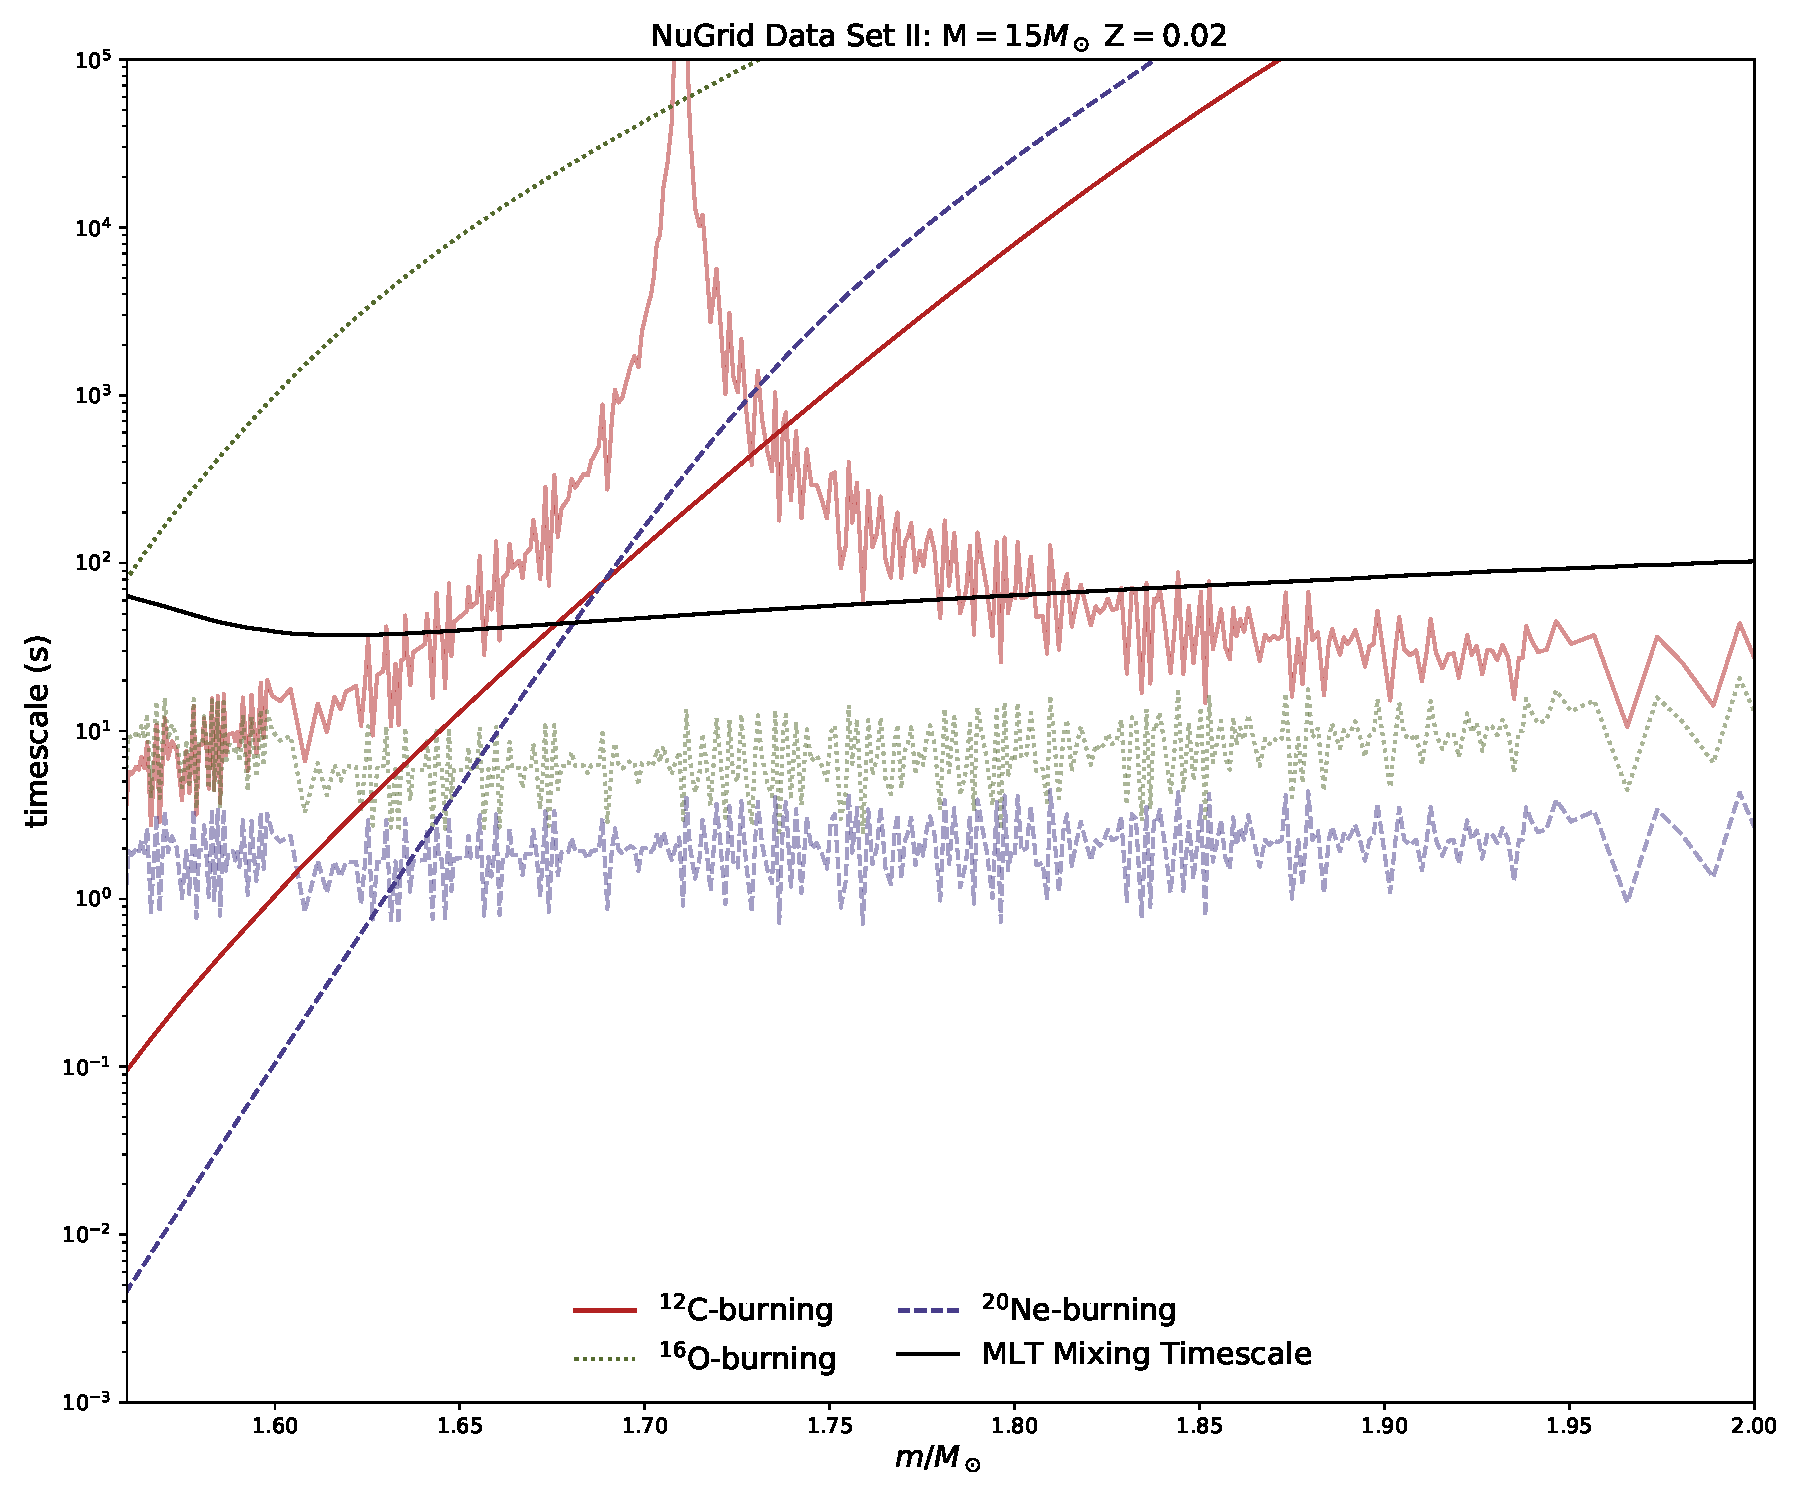
\includegraphics[width=\textwidth]{chapters/1/figures/timescales.pdf}
\caption{Timescales of mixing and burning during the O-C shell merger of a $15 M_\odot$ $Z=0.02$ stellar model from \cite{ritterNuGridStellarData2018} at model number 9200. The black line show the timescale from MLT mixing. The solid red line shows the timescale for a variety of $^{12}\mathrm{C}$ burning reactions and the jagged red line is its corresponding reaction scale height timescale. The dotted green line shows the timescale for a variety of $^{16}\mathrm{O}$ burning reactions and the jagged green line is its corresponding reaction scale height timescale. The dashed blue line shows the timescale for a variety of $^{20}\mathrm{Ne}$ burning reactions and the jagged blue line is its corresponding reaction scale height timescale.}
\label{fig:ritter_timescales}
\end{figure}

As shown in Figure \ref{fig:ritter_timescales}, the timescales for convective mixing and C- and Ne- nuclear burning are comparable, leading to the possibility of different nucleosynthesis pathways occurring in the same zone.
In addition to this, Figure \ref{fig:ritter_timescales} shows how the timescales for a reaction scale height are also comparable to the burning timescale.